\chapter{Model Design and Simulation}
\label{ch:model}

This chapter illustrates the theoretical steps of design, control and simulation of the robotic system. The analysis
deliberately focuses on the developement of a single leg of a hexapod robot.

This strategic choice adheres to a modular approach, which is convenient for several reasons.
Firstly, it ensures that the design can be easily extended and replicated for the remaining limbs, simplifying
the eventual future assembly of the complete robot. Secondly, isolating the study to a single leg allows for a
concentrated focus on the fundamental kinematic and control aspects, thereby optimizing the analysis and
limiting system complexity and implementation time.

\section{Structural Design}

The robotic leg is conceived as a three degrees of freedom (3-DOF) manipulator, a common simplification
of an insect's limb, designed to provide sufficient motion versatility within a robust and manageable structure.
The kinematic chain consists of three rigid links — Coxa, Femur, and Tibia — connected sequentially by three
revolute joints (from the robot's body toward the end-effector, as shown in Figure \ref{fig:hexapod_leg}):

\begin{itemize}
    \item \textbf{Hip Joint} ($q_1$): Connects the robot's body to the Coxa link and primarily controls the
        \textbf{yaw} motion of the leg, responsible for the lateral sweep relative to the body's longitudinal axis.
    \item \textbf{Knee Joint} ($q_2$): Connects the Coxa link to the Femur link and controls the
        \textbf{primary pitch} motion, enabling the lifting and lowering of the leg structure.
    \item \textbf{Ankle Joint} ($q_3$): Connects the Femur link to the Tibia link and controls the
        \textbf{secondary pitch} motion, significantly influencing the height and reach of the Foot (end-effector).
\end{itemize}

This configuration, is widely adopted in hexapod designs as it provides an optimal balance between complexity
and dexterity, allowing for effective gait planning and stable locomotion on various surfaces.

\begin{figure}[htbp]
    \centering
    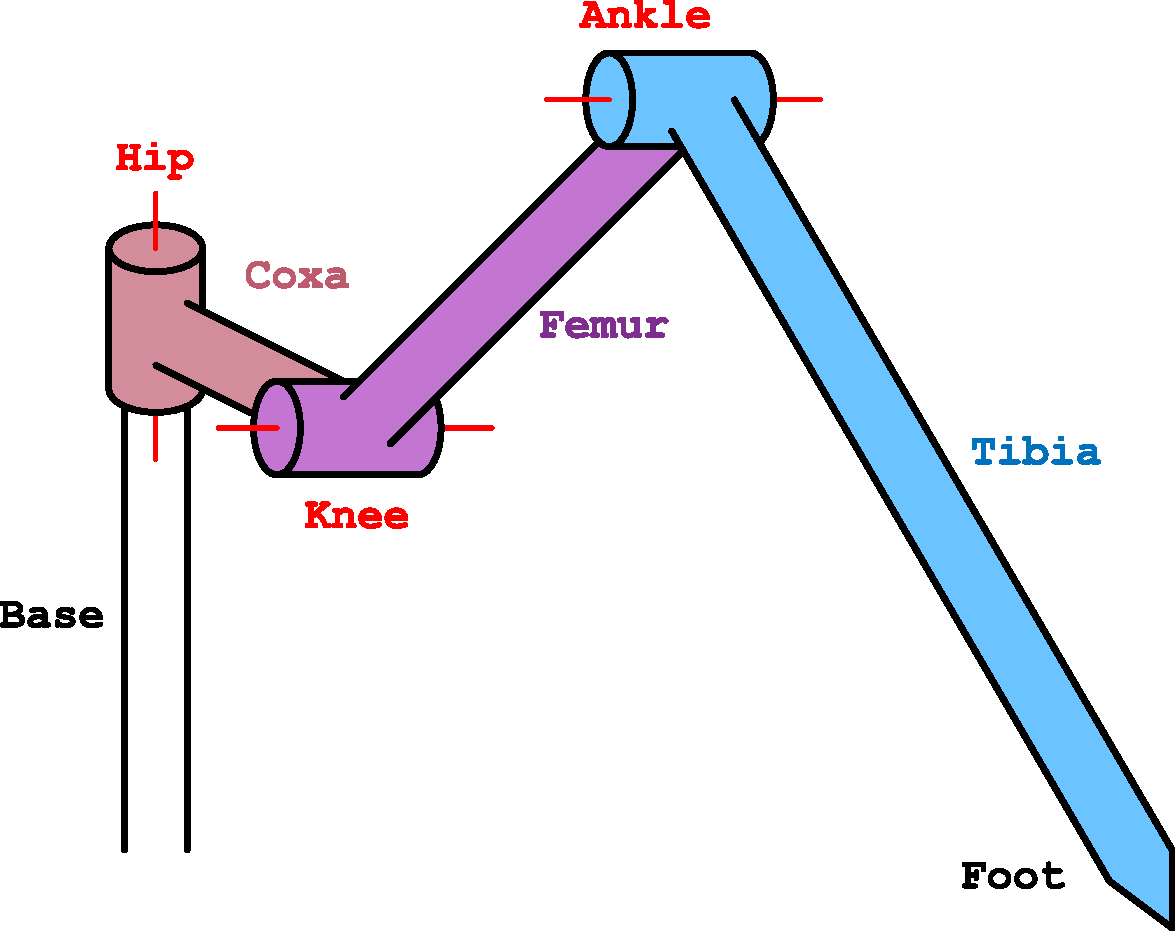
\includegraphics[width=0.8\textwidth]{images/hexapod-leg.pdf}
    \caption{Schematic Representation of the Mechanical Limb}
    \label{fig:hexapod_leg}
\end{figure}


\subsection{Limb Parametrization and Forward Kinematics}
\label{sec:dh_params}

The Denavit--Hartenberg (DH) convention \cite{denavit1955kinematic, siciliano2009robotics} is the standard
mathematical tool for describing the spatial relationships and defining the minimal parameter set required for
kinematic analysis of serial manipulators. By rigidly attaching coordinate frames to each link, DH enables a
standardized description of the link geometry and joint configuration.

The assignment of these frames follows a systematic methodology designed to isolate the four key parameters.
For a kinematic chain starting from a base frame $\{0\}$, a coordinate frame $\{i\}$ is rigidly attached to
link $i$. The most important rule is that the $z_i$-axis is placed along the axis of actuation (either
rotation or translation) for joint $i$. The $x_i$-axis is then constructed along the common normal connecting
$z_{i-1}$ (the previous joint axis) to $z_i$ (the current joint axis), with the origin of frame $\{i\}$
located at the intersection of $x_i$ and $z_i$. Finally, the $y_i$ axis is simply set to complete a
right-handed coordinate system.

Using this precise, rule-based placement of axes the entire transformation from frame $\{i\}$ to frame $\{i+1\}$
can now be described by a sequence of four fundamental operations tied directly to this geometry: the Link Length
($a_i$), Link Twist ($\alpha_i$), Link Offset ($d_i$), and the Joint Angle ($\theta_i$) (see Figure
\ref{fig:denavit_hartenberg}).

\begin{figure}[htbp]
    \centering
    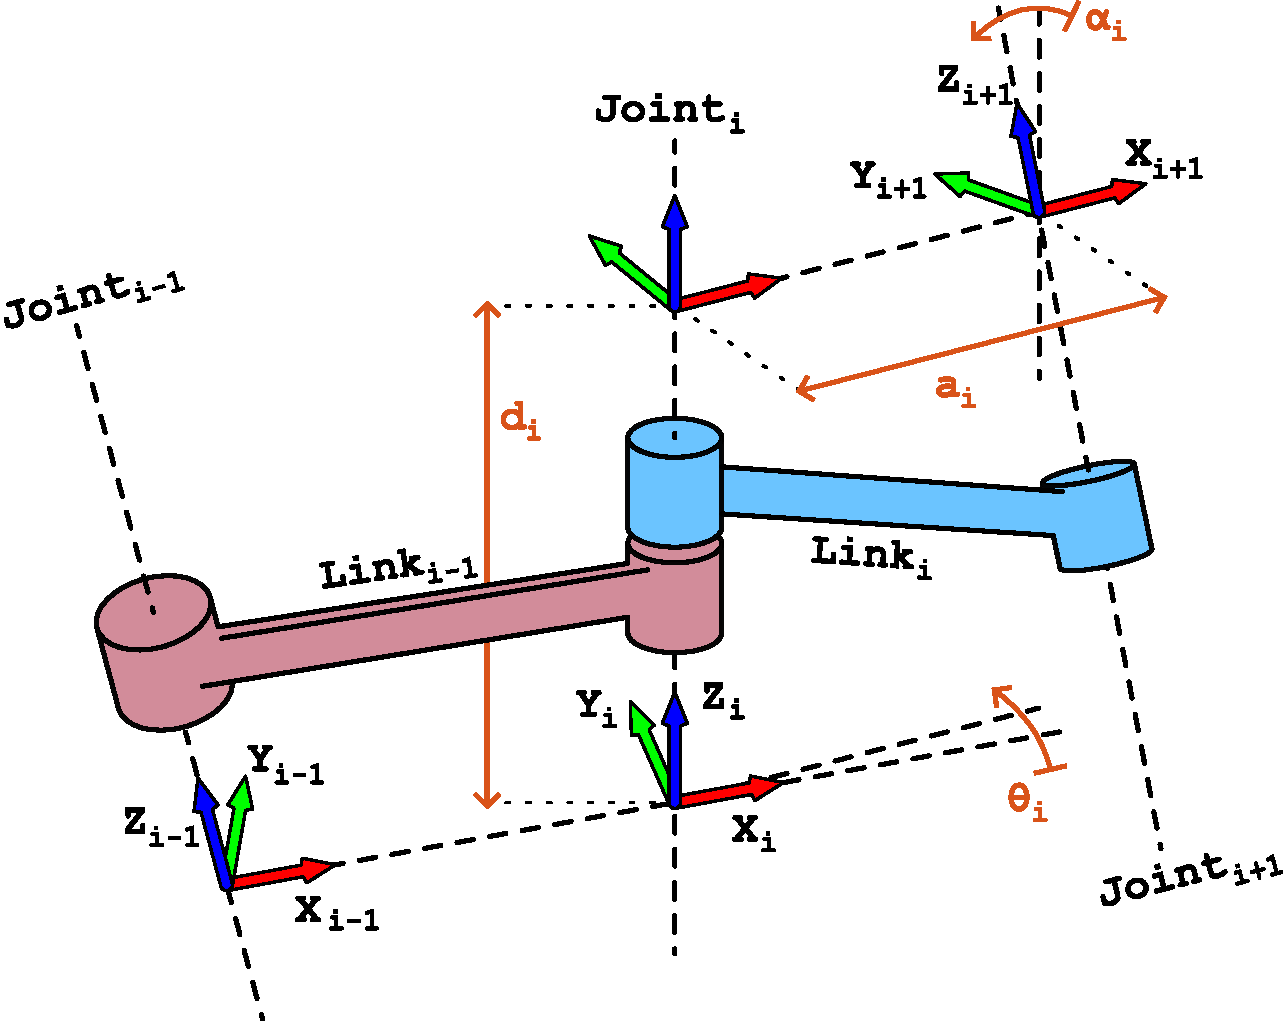
\includegraphics[width=0.8\textwidth]{images/denavit-hartenberg.pdf}
    \caption{Illustration of Denavit--Hartenberg Convention Parameters}
    \label{fig:denavit_hartenberg}
\end{figure}

The homogeneous transformation matrix, $T_{i}^{i+1}$, from frame $\{i\}$ to frame $\{i+1\}$, is given by:

\begin{equation}
    T_{i}^{i+1} = R_x(\alpha_i) \cdot T_x(a_i) \cdot R_z(\theta_i) \cdot T_z(d_i) =
    \begin{bmatrix}
        c_{\theta} & -s_{\theta} & 0 & a \\
        s_{\theta} c_{\alpha} & c_{\theta} c_{\alpha} & -s_{\alpha} & -ds_{\alpha} \\
        s_{\theta} s_{\alpha} & c_{\theta} s_{\alpha} & c_{\alpha} & dc_{\alpha} \\
        0 & 0 & 0 & 1
    \end{bmatrix}
\end{equation}

where the contracted notation $c_x = \cos(x), s_x = \sin(x)$ was used, while the overall transformation from
the base frame $\{b\}$ to the end-effector frame $\{e\}$, $T_b^e$, which is the Forward Kinematics solution,
is computed by the serial multiplication of these individual matrices:

\begin{equation}
    T_b^e = T_b^1 T_1^2 \dots T_{n-1}^n T_n^e
    \label{eqn:transf_matrix}
\end{equation}

To formally derive the Forward Kinematic model of the 3-DOF robotic limb, we apply the DH convention, following
the methodology introduced in the previous section. The assignment of the reference frames is shown in Figure
\ref{fig:assign_dh}, where the $z$-axes are represented in blue, $x$-axes in red and the $y$-axes are omitted.

Frame $\{b\}$ serves as the fixed base frame. In the context of a complete mobile hexapod, this frame is
typically attached to the center of the robot's main body to facilitate gait planning relative to the body's
center of gravity. However, for the experimental verification of the single modular limb in a benchtop setup,
frame $\{b\}$ is rigidly attached to the stationary mounting base, establishing a fixed reference for all
subsequent transformations.

\begin{figure}[htbp]
    \centering
    \begin{subfigure}[c]{0.48\textwidth}
        \centering
        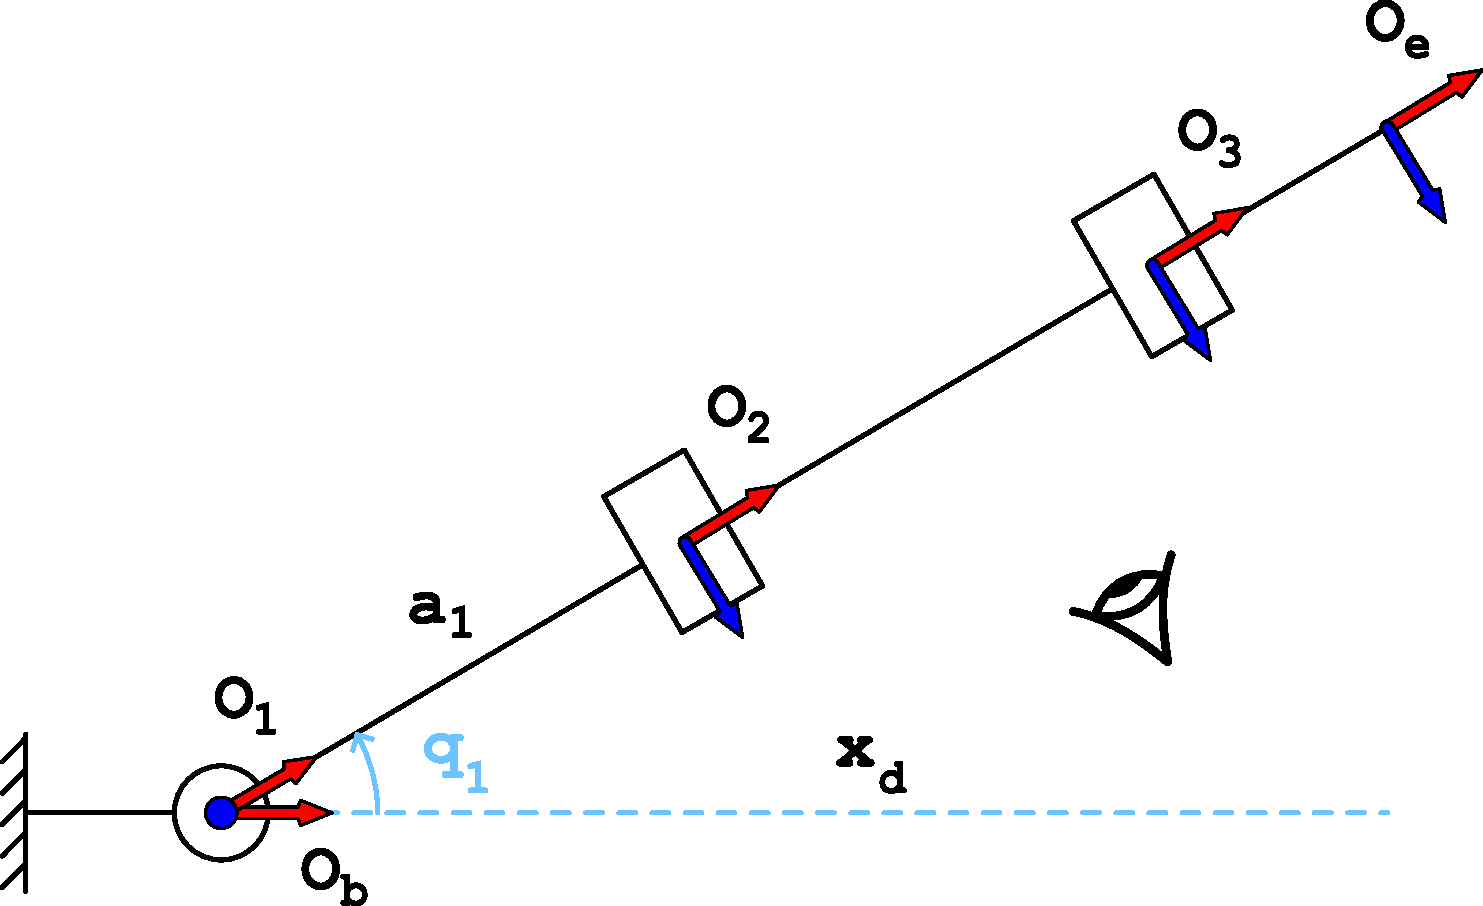
\includegraphics[width=\textwidth]{images/leg-top-dh.pdf}
        \caption{Top View}
        \label{fig:dh_top}
    \end{subfigure}
    \hfill
    \begin{subfigure}[c]{0.48\textwidth}
        \centering
        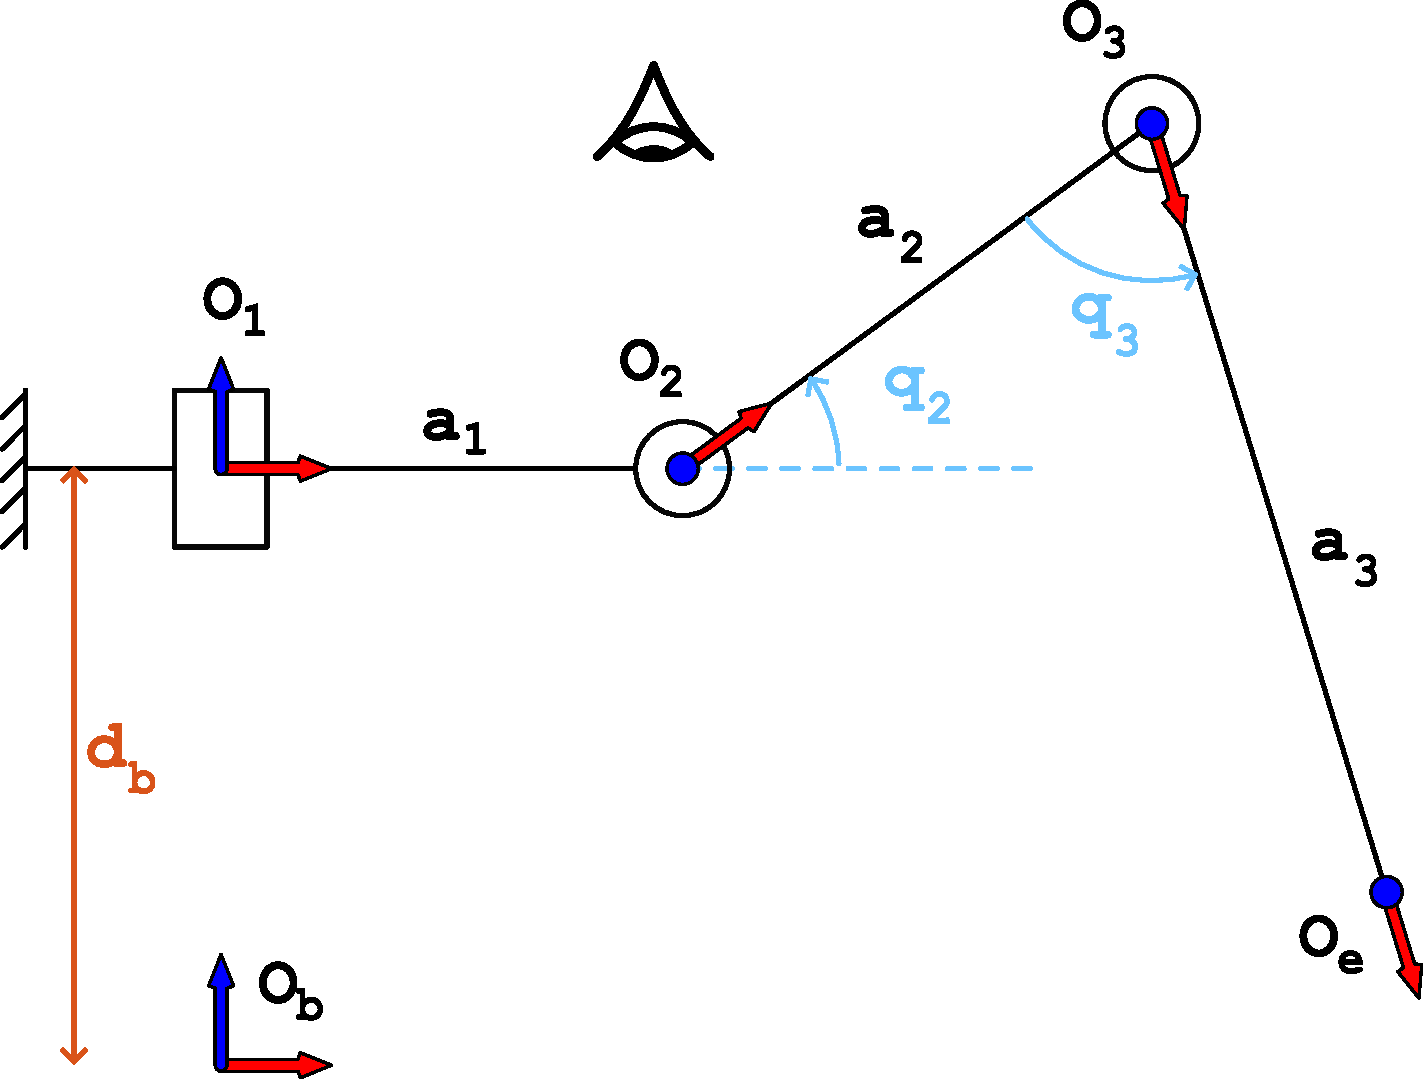
\includegraphics[width=\textwidth]{images/leg-side-dh.pdf}
        \caption{Side View}
        \label{fig:dh_side}
    \end{subfigure}
    \caption{Reference Frames and DH Parameters}
    \label{fig:assign_dh}
\end{figure}

Note the following key design choices:

\begin{itemize}
    \item The base offset $d_b$ represents the distance from the base frame $\{b\}$ to the frame of the Hip Joint
        (i.e. the mounting height of the leg on the base).
    \item The link lengths $a_1$, $a_2$ and $a_3$ correspond to the length of the Coxa, Femur and Tibia links,
        respectively. These values are chosen based on a mix of aesthetics and physical constraints. More
        specifically, the Coxa length is minimized and the Femur length is chosen to be smaller than the Tibia
        length.
    \item The twist angle $\alpha_1 = 90^{\circ}$ is necessary because the axis of the Knee Joint ($z_2$) is
        orthogonal to the axis of the Hip Joint ($z_1$).
    \item Subsequent frames are coplanar, resulting in zero twist angles ($\alpha_2 = \alpha_3 = 0^{\circ}$)
        and link offsets ($d_1 = d_2 = d_3 = 0\ mm$), simplifying the transformation matrices.
    \item The joint angle $q_3$ is rotated by an extra $-180^\circ$ to simplify IK derivation and match the
        hardware implementation.
    \item Since the attitude of the end-effector is irrelevant, the final joint angle for the Tibia link is
        fixed at $\theta_4 = 0$, as the end-effector (Foot) frame $\{e\}$ is placed at the tip of the Tibia
        link, defining the final link length $a_3$.
\end{itemize}

The parameter for the DH model are reported in Table \ref{tab:dh_parameters}.

\begin{table}[htbp]
    \centering
    \begin{tabular}{c c c c c}
        \hline
        \textbf{Link} & \textbf{$a$ [mm]} & \textbf{$\alpha$ [deg]} & \textbf{$d$ [mm]} & \textbf{$\theta$ [deg]} \\
        \hline
        \hline
        Base    & $0$           & $0$   & $d_b = 178$   & $q_1$         \\
        Coxa    & $a_1 = 40$    & $90$  & $0$           & $q_2$         \\
        Femur   & $a_2 = 78$    & $0$   & $0$           & $q_3 - 180$   \\
        Tibia   & $a_3 = 132$   & $0$   & $0$           & $0$           \\
        \hline
    \end{tabular}
    \caption{Denavit--Hartenberg Parameters of the Limb}
    \label{tab:dh_parameters}
\end{table}


\subsection{Inverse Kinematics Overview and Derivation}

Forward Kinematics analysis allows for the straightforward computation of the end-effector's pose starting from a
known joint configuration. However, this direct mapping is often impractical for high-level control. Defining a
task or a trajectory is inherently more intuitive in Cartesian space (e.g. coordinates in the world frame) than
in the abstract joint space. Consequently, to command the robot to reach a specific physical location, the
inverse problem must be addressed.

Inverse Kinematics (IK) \cite{siciliano2009robotics} is the problem of determining the set of joint variables,
$q = [q_1, \dots, q_n]$, required to place the end-effector at a desired pose, $p_d = [x_d, y_d, z_d, \phi_d, \theta_d, \psi_d]^T$.
Unlike Forward Kinematics, the IK problem is fundamentally more challenging due to the non-linear relationship
between joint space and Cartesian space. The mathematical objective is to solve the inverse mapping:
\begin{equation*}
    q = f^{-1}(p_d)
\end{equation*}

The complexity of the problem stems from several factors. Solutions may be non-unique, meaning multiple
joint configurations can achieve the same end-effector pose and/or non-existent if the target pose lies outside
the robot's physical workspace. Furthermore, singularities — joint configurations that cause a loss of effective
degrees of freedom — must be avoided as they lead to control instability.

To address these challenges, solution approaches usually fall into two main categories: on one side, analytical
solutions provide closed-form, explicit equations for the joint variables as a function of the desired pose,
offering high computational efficiency and usually providing all possible solutions. They are generally preferred
for manipulators with simple geometries. Numerical Methods, conversely, use iterative algorithms to converge on a
solution by minimizing a position error function. While they are necessary for complex kinematic structures
lacking analytical solutions, they are less computationally efficient and provide only one solution per iteration.

Given the simple structure of the application, an analytical solution can be found using planar geometry and
fundamental trigonometric relationships. For the derivation, the leg geometry is conceptually separated into two
different point of views, to facilitate the calculation. Figure \ref{fig:find_ik} depicts a schematic representation
of them.

\begin{figure}[htbp]
    \centering
    \begin{subfigure}[t]{0.48\textwidth}
        \centering
        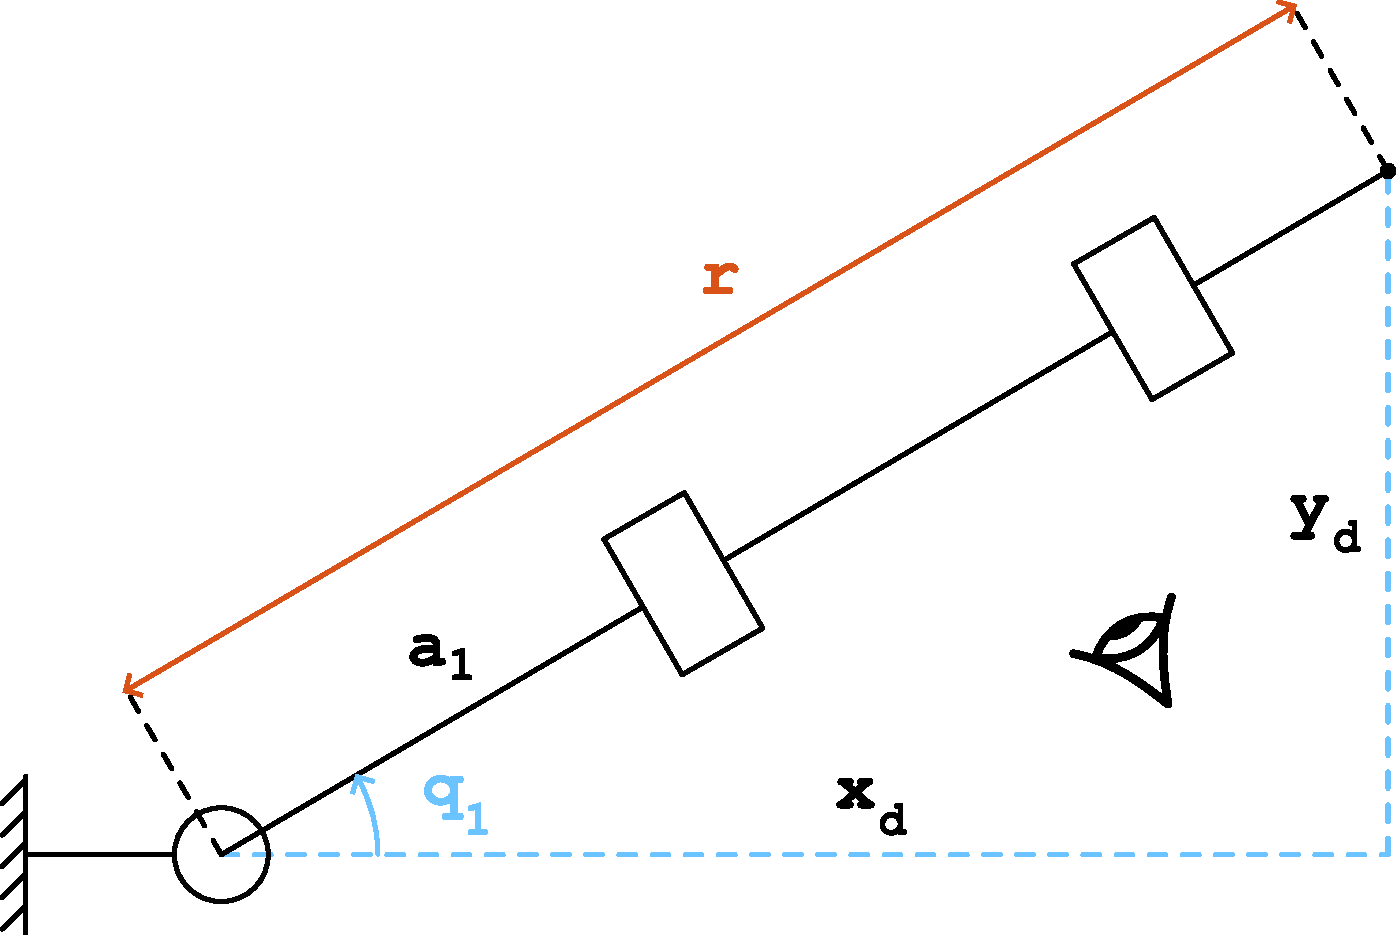
\includegraphics[width=\textwidth]{images/leg-top-ik.pdf}
        \caption{Top View}
        \label{fig:ik_top}
    \end{subfigure}
    \hfill
    \begin{subfigure}[t]{0.48\textwidth}
        \centering
        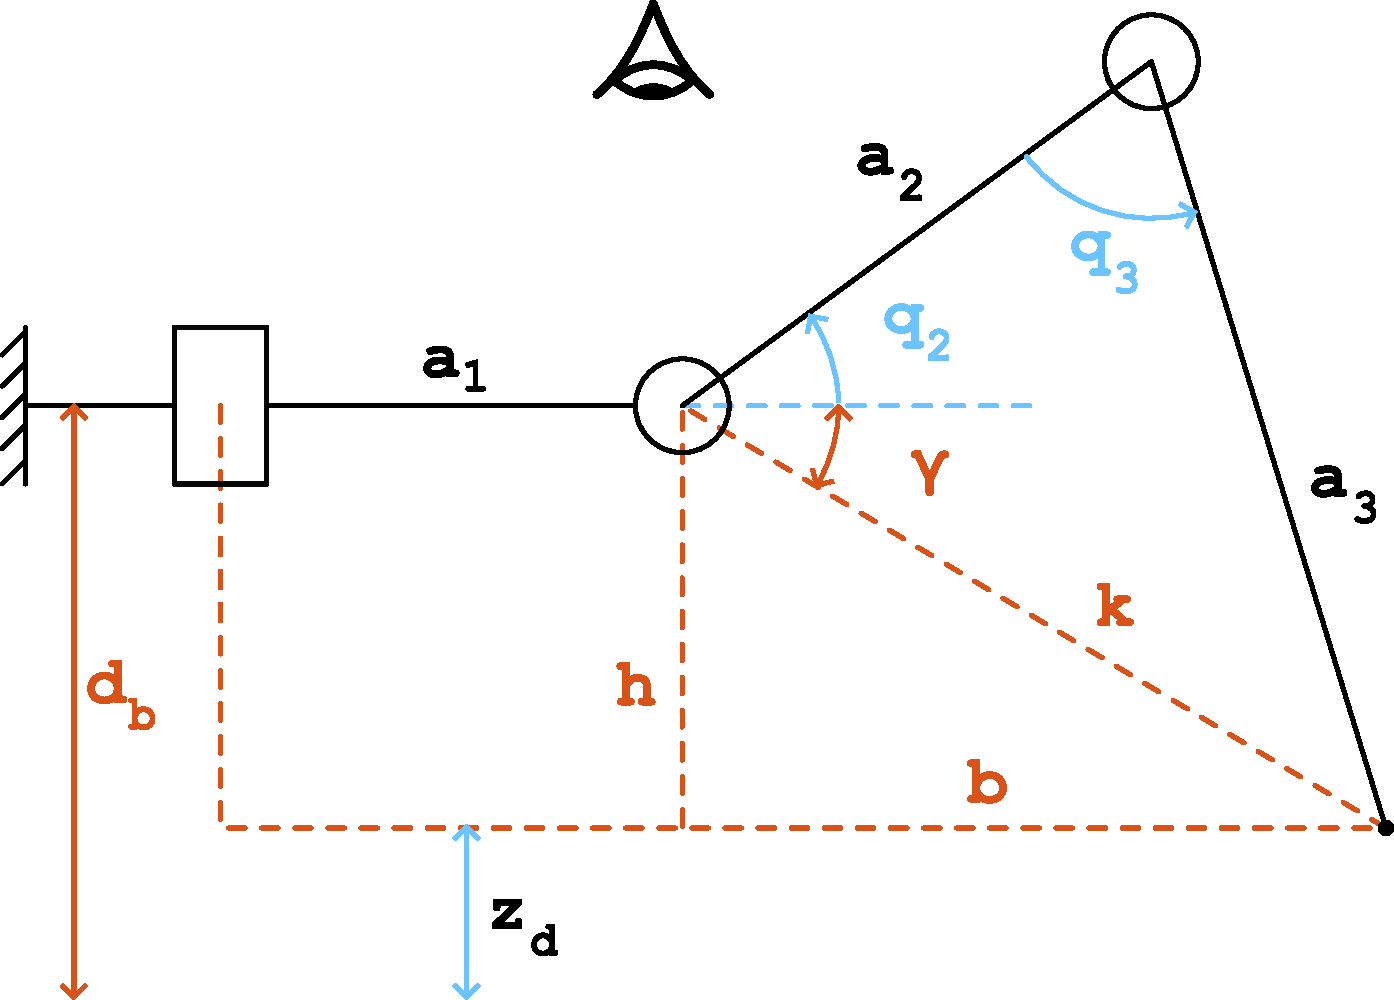
\includegraphics[width=\textwidth]{images/leg-side-ik.pdf}
        \caption{Side View}
        \label{fig:ik_side}
    \end{subfigure}
    \caption{Leg Geometry for IK Derivation}
    \label{fig:find_ik}
\end{figure}

Given a desired end-effector position $p_d = [x_d, y_d, z_d]^T$, the three required joint angles $q_1, q_2, q_3$
can be determined sequentially as follows:


\subsubsection{Joint Angle $q_1$ (Yaw)}

The first joint angle, $q_1$, is determined solely by the $X$ and $Y$ coordinates of the desired position,
representing a rotation in the horizontal plane (Figure \ref{fig:ik_top}). This is a straightforward calculation:
\begin{equation*}
    q_1 = \operatorname{atan2}(y_d,x_d)
\end{equation*}
The $\operatorname{atan2}$ function ensures that the resulting angle correctly accounts for the sign of the
coordinates across all four quadrants, providing the correct angle $\theta \in [-\pi, \pi]$.


\subsubsection{Joint Angles $q_2$ and $q_3$ (Pitch)}

The derivation of $q_2$ and $q_3$ is performed in the vertical plane (Figure \ref{fig:ik_side}),
which is defined by the Femur and Tibia links. We first define a set of auxiliary geometric variables:
\begin{itemize}
    \item \textbf{Projected Radial Distance ($r$):} The distance from the origin to the end-effector projected
        onto the $XY$-plane.
        \begin{equation*}
            r = \sqrt{x_d^2 + y_d^2}
        \end{equation*}
    \item \textbf{Horizontal Distance ($b$):} The effective horizontal distance from the $q_2$ joint axis to
        the end-effector.
        \begin{equation*}
            b = r - a_1 \Leftarrow r = b + a_1
        \end{equation*}
    \item \textbf{Vertical Distance ($h$):} The effective vertical distance from the $q_2$ joint axis to
        the end-effector.
        \begin{equation*}
            h = d_b - z_d
        \end{equation*}
    \item \textbf{Virtual Link Length ($k$):} The length of the virtual link connecting the $q_2$ joint axis
        to the end-effector, forming the third side of the triangle with links $a_2$ and $a_3$.
        \begin{equation*}
            k = \sqrt{h^2 + b^2}
        \end{equation*}
    \item \textbf{Knee Offset Angle ($\gamma)$:} The angle between the continuation of $a_1$ and the
        virtual link length $k$.
        \begin{equation*}
            \gamma = \operatorname{atan2}(h, b)
        \end{equation*}
        Using $\operatorname{atan2}$ ensures once again correctness even when $h$ is negative, i.e. when the
        Foot is above the body of the robot.
\end{itemize}

Using these auxiliary variables, the final joint angles $q_2$ and $q_3$ can now be obtained.

The second joint angle, $q_2$, is found by determining the internal angle of the $a_2, a_3, k$ triangle
using the Law of Cosines and compensating for the angle ($\gamma$):
\begin{equation*}
    q_2 = \operatorname{acos}\left(\frac{a_2^2 + k^2 - a_3^2}{2 \cdot a_2 \cdot k}\right) - \gamma
\end{equation*}
The third and final joint angle, $q_3$, is the angle between the $a_2$ and $a_3$ links. This is again derived
from the Law of Cosines:
\begin{equation*}
    q_3 = \operatorname{acos}\left(\frac{a_2^2 + a_3^2 - k^2}{2 \cdot a_2 \cdot a_3}\right)
\end{equation*}

Substituting the intermediate variables back into the expressions for $q_2$ and $q_3$ yields the final,
consolidated IK equations as a direct function of the desired end-effector coordinates as reported in Appendix
\ref{app:ik}.

\section{Reachable Workspace and Path Planning}
\label{sec:trajectory}

Following the developement of the limb's kinematic model, the next logical step is to verify the correctness of
the design and its behaviour through digital simulation. However, two preliminary steps are essential: the reachable
workspace of the system must be analyzed to understand its operational boundaries and a desired trajectory for the
end-effector must be designed.


\subsection{Workspace Definition and Analysis}

The reachable workspace of a manipulator is formally defined as the complete set of all Cartesian positions
$p = [x,y,z]^{T}$ that its end-effector can attain, given the physical constraints of its kinematic
chain \cite{ding2010locomotion}. It represents the entire volume of space accessible to the robot's
end-effector. For this 3-DOF limb, the workspace is determined by the three link lengths ($a_{1},a_{2},a_{3}$)
and, most critically, by the actuation limits imposed on its three joints ($q_{1},q_{2},q_{3}$).

To characterize this 3D volume, a two-stage approach is taken. First, the 2D planar workspace is analyzed.
This is done by fixing the Hip Joint at a neutral angle (e.g. $q_1 = \ang{0}$) and generating the boundary of
the leg's reach in a single vertical plane. A 2D cross-section is then obtained by sweeping the Knee
($q_2$) and Ankle ($q_3$) joints through their entire operational ranges. The resulting surface (Figure
\ref{fig:workspace_analysis}) is finally revolved around the Hip joint axis by sweeping $q_1$ through its own
range, thereby generating the final 3D reachable volume.

\begin{figure}[htbp]
    \centering
    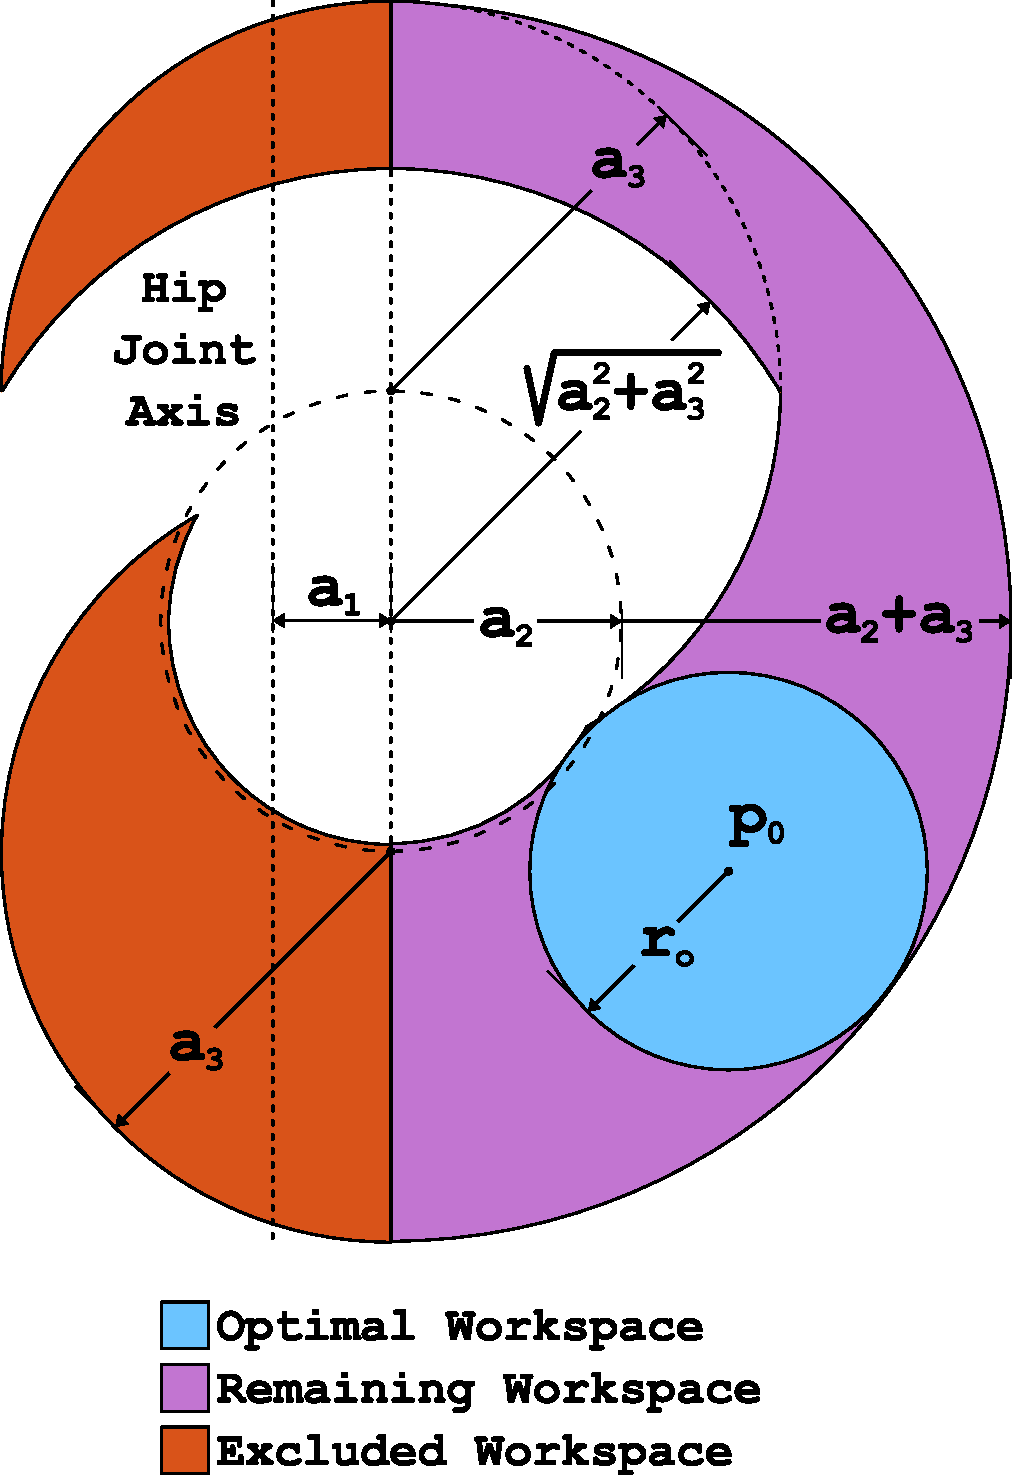
\includegraphics[width=0.7\textwidth]{images/workspace.pdf}
    \caption{Reachable Workspace Section for $q_1 = 0$}
    \label{fig:workspace_analysis}
\end{figure}

The actuator limits are the primary constraints defining this space. These limits are imposed both by the
physical components (i.e. the finite rotational range of the servo-motors) and by the mechanical design itself,
which is configured to prevent self-collision between links and other limbs.
For this specific implementation, the joint constraints are defined as follows:
\begin{equation*}
  q =[q_1, q_2, q_3]^T \in
  \left[-30^\circ, 30^\circ \right]
  \times
  \left[-90^\circ, 90^\circ \right]
  \times
  \left[30^\circ, 180^\circ \right]
\end{equation*}

As an additional safety measure, a portion of the resulting workspace (the red coloured area in Figure
\ref{fig:workspace_analysis}) is excluded from operation to prevent collisions with the robot's body or the mounting
structure. A simplified and safe \textbf{Optimal Work Region} is then defined by inscribing a sphere within the
remaining viable workspace depicted in blue. The center of this sphere, $p_0$, is designated as the leg's nominal
\textbf{Rest Position}, which will serve as the origin for gait trajectories.


\subsection{Trajectory Design}

Moving to trajectory generation, the goal is to create a function $p_d$ to define the motion of the foot.
The design of this trajectory is guided by several key principles and assumptions. Firstly, the path
must be parametric, dependent on both the desired walking speed $v$ and the direction of movement $\psi$.
Secondly, the trajectory primitive is generated relative to the leg's central rest position $p_0$, which is
eventually added as a final offset to determine the absolute path $p_d(t)$. For this initial derivation, we
also assume the ground is a flat, predictable plane at a constant height set to 0 (or $p_{z,0}$ after applying
the rest offset).

The gait cycle is composed of two distinct and well defined phases, which needs to be properly stitched together
to ensure smooth ($C^2$) motion. During the \textbf{Stance Phase}, the foot must remain stationary relative to
the ground as the body moves forward. This implies that the foot's velocity relative to the robot's body must
be constant and equal to $-v$ (along the $\psi$ direction). Consequently, the acceleration during this linear
phase is zero. Conversly, during the \textbf{Swing Phase}, the leg should relocate to start a new cycle
while also lifting off the ground.


\subsubsection{Quintic Polynomials}

The simplest and most widely adopted solution in robotics is using fifth-order (quintic) polynomials
\cite{biagiotti2008trajectory, siciliano2009robotics} to move between two points while matching boundary
conditions for position, velocity, and acceleration. A generic quintic polynomial is defined by six
coefficients ($c_0, \dots, c_5$):

$$ p(t) = c_5t^5 + c_4t^4 + c_3t^3 + c_2t^2 + c_1t + c_0 $$

The function $p(t)$ represents the position, while its first and second time derivatives, $v(t)$ and $a(t)$,
represent the velocity and acceleration, respectively:

$$ v(t) = \frac{dp}{dt} = 5c_5t^4 + 4c_4t^3 + 3c_3t^2 + 2c_2t + c_1 $$
$$ a(t) = \frac{d^2p}{dt^2} = 20c_5t^3 + 12c_4t^2 + 6c_3t + 2c_2 $$

To solve for the six unknown coefficients $\mathbf{c} = [c_0, c_1, c_2, c_3, c_4, c_5]^T$, we impose six
known boundary conditions, i.e. the desired position, velocity, and acceleration at the start time ($t = 0$)
and at the end time ($t = T$), where $T$ is the total duration of the movement. Then a system of six linear
equations can be derived and expressed in matrix form as $M \cdot \mathbf{c} = \mathbf{b}$:

$$
  \begin{bmatrix}
    1 & 0 & 0 & 0 & 0 & 0 \\
    0 & 1 & 0 & 0 & 0 & 0 \\
    0 & 0 & 2 & 0 & 0 & 0 \\
    1 & T & T^2 & T^3 & T^4 & T^5 \\
    0 & 1 & 2T & 3T^2 & 4T^3 & 5T^4 \\
    0 & 0 & 2 & 6T & 12T^2 & 20T^3
  \end{bmatrix}
  \begin{bmatrix}
    c_0 \\ c_1 \\ c_2 \\ c_3 \\ c_4 \\ c_5
  \end{bmatrix}
  =
  \begin{bmatrix}
    p_0 \\
    v_0 \\
    a_0 \\
    p_f \\
    v_f \\
    a_f
  \end{bmatrix}
$$

The vector of coefficients $\mathbf{c}$ can then be found by inverting the $6 \times 6$ matrix $M$ and
multiplying it by the vector of boundary conditions $\mathbf{b}$:

\begin{equation}
  \mathbf{c} = M^{-1} \cdot \mathbf{b}
  \label{eqn:quintic_poly_solution}
\end{equation}

The resulting coefficients are constants that depend only on the specified boundary conditions and the total
movement time $T$. The final trajectory $p(t)$ is then a continuous function of the generic time variable
$t \in [0, T]$.


\subsubsection{Horizontal Component}

We start by defining the 1D horizontal component of the trajectory, $p_h(t)$, as a function of normalized time
$t \in [0, 1]$, and representing the motion along the direction of travel $\psi$. The 2D path in the $XY$ plane
is simply this 1D motion projected onto the direction vector $\mathbf{d}(\psi) = [\sin(\psi), \cos(\psi)]^T$.

We define the \textbf{Duty Factor} $\beta$ as the fraction of the cycle spent in the Stance Phase (typically
$\beta > 0.5$ for structural stability, meaning that the robot is supported by at least 3 contact points at every
moment). This divides the normalized unit period into two segments:

$$ T_{stance} = \beta $$
$$ T_{swing} = (1-\beta) $$

The cycle is thus defined with the Swing Phase occurring for $t \in [0, T_{swing}]$ and the Stance Phase for
$t \in [T_{swing}, 1]$. The trajectory oscillates between a forward limit (touchdown) $p_1 = r$ and a backward
limit (liftoff) $p_2 = -r$. The total horizontal stroke is $S = 2r$.

During the Stance Phase, the motion is linear, connecting the touchdown point (at $t = T_{swing}$, $p = r$) to
the liftoff point (at $t = 1$, $p = -r$). The function $p_{h,stance}(t)$ is the equation of this line. Its slope,
the normalized velocity $v_{norm}$ is constant:

$$ v_{norm} = \frac{\Delta p}{\Delta t} = \frac{-2r}{\beta} $$
The trajectory for this phase and its derivatives are given by:
$$ p_{h,stance}(t) = p_1 + v_{norm} \cdot (t - T_{swing}) $$
$$ v_{h,stance}(t) = v_{norm} $$
$$ a_{h,stance}(t) = 0 $$
During the Swing Phase, we use the quintic polynomial method to move from the liftoff position back to the
touchdown position. This function must smoothly connect the end of the previous stance phase (at $t = 1$,
or $t = 0$ in the new cycle) to the start of the current stance phase (at $t = T_{swing}$).

To ensure $C^2$ continuity, we must match the position, velocity, and acceleration of the stance phase at both
ends. We solve for the polynomial $p_{h,swing}(t)$ over the interval $T = T_{swing}$ using the following
boundary conditions vector $\mathbf{b}_{h,swing} = [-r, v_{norm}, 0, r, v_{norm}, 0]^T$.
Solving Equation \ref{eqn:quintic_poly_solution} with this vector yields the specific coefficients for the
horizontal swing polynomial.


\subsubsection{Vertical Component}

Next, we define the vertical component of the motion, $p_z(t)$, relative to the ground plane.

During the stance phase the foot is on the ground providing propulsion, therefore $p_{z,stance}(t) = 0$. This
implies $v_{z,stance} = 0$ and $a_{z,stance}(t) = 0$.

During the swing phase, the leg must lift to a clearance height $H_{lift}$ ($= r$) and return to the ground.
This motion must also be $C^2$ continuous, connecting smoothly to the zero-motion of the Stance Phase. To
achieve this, the Swing Phase is split into two identical halves, "Lift-Up" and "Lift-Down", each with duration
$T_{lift} = T_{swing} / 2$.

We solve for the lift-up polynomial $p_{z,up}(t)$. The boundary conditions must match the stance phase at the
start ($t = 0$) and ensure a smooth apex at the peak ($t = T_{lift}$). The boundary conditions vector is
$\mathbf{b}_{z,up} = [0, 0, 0, H_{lift}, 0, 0]^T$. Then, the lift-down polynomial is a time-mirrored version of
the lift-up segment.

This two-stage approach guarantees $C^2$ continuity for the entire vertical trajectory: it starts from
$p=0, v=0, a=0$ (matching the stance end), achieves a smooth peak at $t = T_{lift}$, and returns to
$p=0, v=0, a=0$ at $t = T_{swing}$ (matching the stance start).


\subsubsection{Path Assembly}

The complete spatial geometry of the gait, $p_{prime}(t)$ is now fully designed, as a function of the
normalized time $t \in [0, 1]$. The complete primitive is assembled by combining the horizontal and vertical
components, projecting the horizontal motion onto the $X$ and $Y$ axes, and stitching the swing and stance
phases together:
$$
p_{prime}(t) =
  \begin{cases}
    \begin{bmatrix}
      p_{h,swing}(t) \sin(\psi) \\
      p_{h,swing}(t) \cos(\psi) \\
      p_{z,swing}(t)
    \end{bmatrix}
    & \text{Swing: } 0 \le t < T_{swing} \\
    \\
    \begin{bmatrix}
      p_{h,stance}(t) \sin(\psi) \\
      p_{h,stance}(t) \cos(\psi) \\
      0
    \end{bmatrix}
    & \text{Stance: } T_{swing} \le t \le 1 \\
  \end{cases}
$$
The desired path $p_d(t)$ sent to the controller is then obtained by biasing this primitive with the
leg's central rest position $p_d(t) = p_0 + p_{prime}(t)$.

Crucially, this formulation decouples the path's spatial geometry from its execution speed.
The function $p_{prime}(t)$ defines only the geometric path, with the input $t$ representing the percentage
of cycle completion, not the actual time.


\subsubsection{Walking Speed Dependance}

The desired physical walking speed $v$ is introduced by controlling how fast this normalized time $t$ advances
in the real world. This is achieved through a discrete-time implementation. First, we determine the required
real-time period ($T_{real}$) for one full gait cycle. The physical stroke $S = 2r$ must be covered at the
desired velocity $v$ during the stance phase, which lasts for a fraction $\beta$ of the total period, therefore
the total real-time period for the cycle is:
$$ T_{real} = \frac{2r}{\beta v} $$
In the control loop, the normalized path $p_{prime}(t)$ is discretized into $n$ samples (e.g. $n = 1000$).
A counter $k$ (where $0 \le k < n$) tracks the current step, and the corresponding normalized time is $t_k = k/n$.
The controller achieves the desired velocity $v$ by incrementing the counter $k$ at a specific real-time
frequency, $f$ determined by the real-time step $\Delta t_{real}$, which is the total period divided by the
number of samples:
$$ \Delta t_{real} = \frac{T_{real}}{n} = \frac{2r}{n \beta v} $$
The controller's update frequency is $f = 1 / \Delta t_{real}$. By adjusting this frequency $f$ (or its inverse,
the time step $\Delta t_{real}$), the desired velocity $v$ is precisely controlled, while the spatial trajectory
remains constant.
\section{Control and Simulation}
\label{sc:simulation}

Having defined the complete kinematic model via the DH parameters, derived the IK solver, and designed a $C^2$
continuous gait trajectory, we proceed to validate the entire system by simulation. To verify that these
theoretical components function correctly in unison, a digital model of the leg is implemented in the
Simulink \cite{matlab} environment. This simulation serves as a crucial proof-of-concept, allowing for the
verification of the control logic and the workspace before committing to physical hardware. This section details
the open-loop control architecture used for this validation and the construction of the simulation model itself.


\subsection{Open Loop Control Strategy}

The control strategy adopts an open-loop architecture (Figure \ref{fig:control_chain}), deliberately neglecting
external disturbances or modeling errors; its sole purpose is to validate the correctness of the kinematic chain.

It consists in:

\begin{itemize}
  \item \textbf{Path Planning:} The Gait Trajectory Generator outputs the desired Cartesian position $p_d(t)$
    at each time step, given a desired walking speed $v$ and direction $\psi$.
  \item \textbf{Inverse Kinematics:} The desired path $p_d(t)$ is fed into the IK solver, which
    calculates the required vector of joint angles $q_d(t) = [q_1, q_2, q_3]^T$ needed to achieve
    that end-effector position.
  \item \textbf{Leg Model (Plant):} The desired angles $q_d(t)$ are sent as commands to the
    digital twin of the leg, modeled with the aid of the Simscape library.
  \item \textbf{Forward Kinematics:} For validation, the actual joint angles from the simulation model are
    fed into the FK block (based on the DH Table \ref{tab:dh_parameters}). This calculates the resulting
    end-effector position, $p_{sim}(t)$.
\end{itemize}

\begin{figure}[htbp]
    \centering
    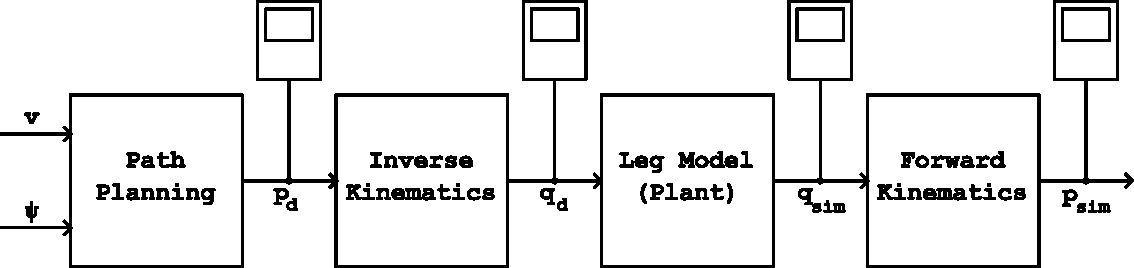
\includegraphics[width=0.98\textwidth]{images/open_loop.pdf}
    \caption{Block Diagram of the Open Loop Control Chain.}
    \label{fig:control_chain}
\end{figure}

A key assumption at this stage is the use of ideal actuators. The joints in the simulation are modeled as
ideal position controllers. This means that when a joint is commanded to go to an angle $q_i$, it achieves
this setpoint almost instantaneously and without error. We are intentionally neglecting the dynamics of the
motors (e.g. torque limits, friction, PID control, and settling time) to isolate the validation purely to the
kinematic model.

The goal is to answer the question: "If the joints go to the angles we calculated, does the foot go to the
position we intended?" The simulation is considered successful if the error between the desired path and the
actual path is approximately close to zero for the entire duration.


\subsection{Digital Simulation}

To create a realistic and physically-grounded representation of the leg, the digital twin is constructed using
Simscape Multibody \cite{simscape}. This MATLAB/Simulink toolbox allows for the modeling of 3D mechanical systems
by defining rigid bodies, joints, constraints, and their spatial relationships.

The leg model (reported in Figure \ref{fig:simscape_model}) is built by importing the CAD (Computer-Aided Design)
files for each link (Coxa, Femur, and Tibia) for a better graphical representation. These rigid bodies are then
connected using 'Revolute Joint' and 'Transformation' blocks at the appropriate locations, corresponding to the
physical actuators and established DH parameters. The joint axes and link-to-link coordinate frames are meticulously
aligned ensuring the simulation model is a one-to-one representation of the theoretical kinematic chain.

\begin{figure}[htbp]
    \centering
    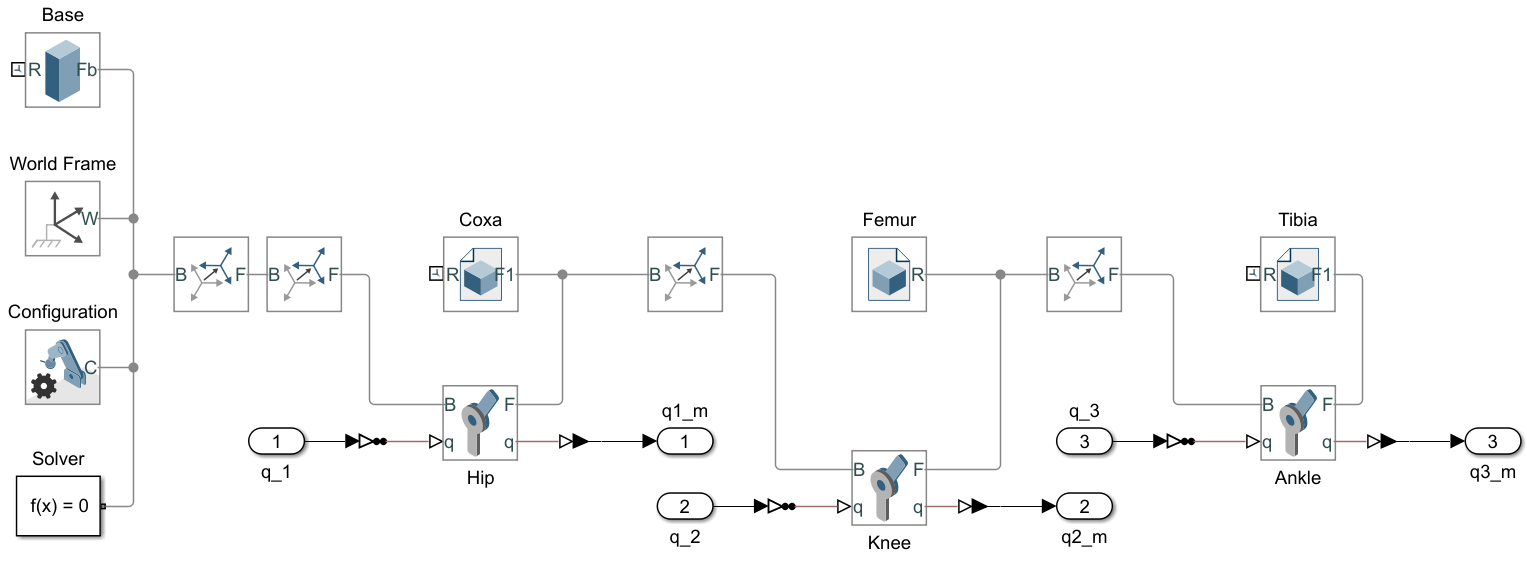
\includegraphics[width=0.98\textwidth]{images/simscape.PNG}
    \caption{Simscape Multibody Limb Model (Plant Block).}
    \label{fig:simscape_model}
\end{figure}

This model serves as the 'Plant' block in the control diagram. The inputs to the model are the three desired
joint angles $q_d(t)$ from the IK block, which drive the 'Sensing and Motion' input of the Revolute
Joint blocks. The outputs are the resulting joint angles and poses, which are passed to the FK validation block
and used to generate the 3D animation (as seen in Figure \ref{fig:rendering_side}) for visual confirmation
of the gait.

\begin{figure}[htbp]
    \centering
    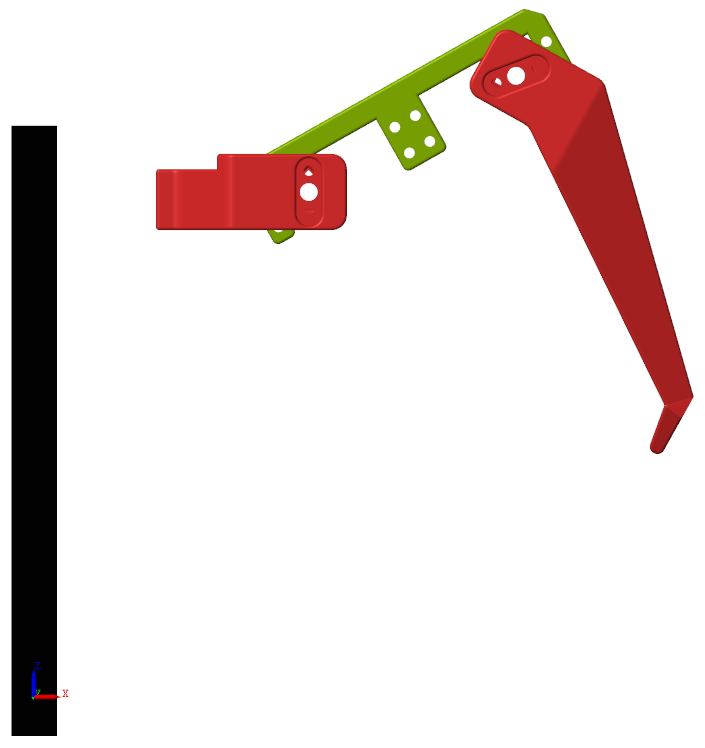
\includegraphics[width=0.48\textwidth]{images/model_side.PNG}
    \caption{3D Rendering of the Simscape Simulation (Side View).}
    \label{fig:rendering_side}
\end{figure}

For the purpose of the digital simulation, the walking direction will be set to be coincident with the y axis
($\vec{\psi} = \vec{y}$).


\subsection{Simulation Results}
\label{sec:simulation_results}

The primary validation of the theoretical model comes from a comparison of the desired Cartesian path (the output
of the Path Generator, $p_d$) against the actual path achieved by the Simscape model (the output of the Forward
Kinematics block, $p_{sim}$). These two trajectories (Figure \ref{fig:gait_z_psi}) are undistinguishable,
confirming the entire kinematic chain — from the DH parameters and IK solver to the FK validation — is
mathematically correct and consistent.

\begin{figure}[htbp]
    \centering
    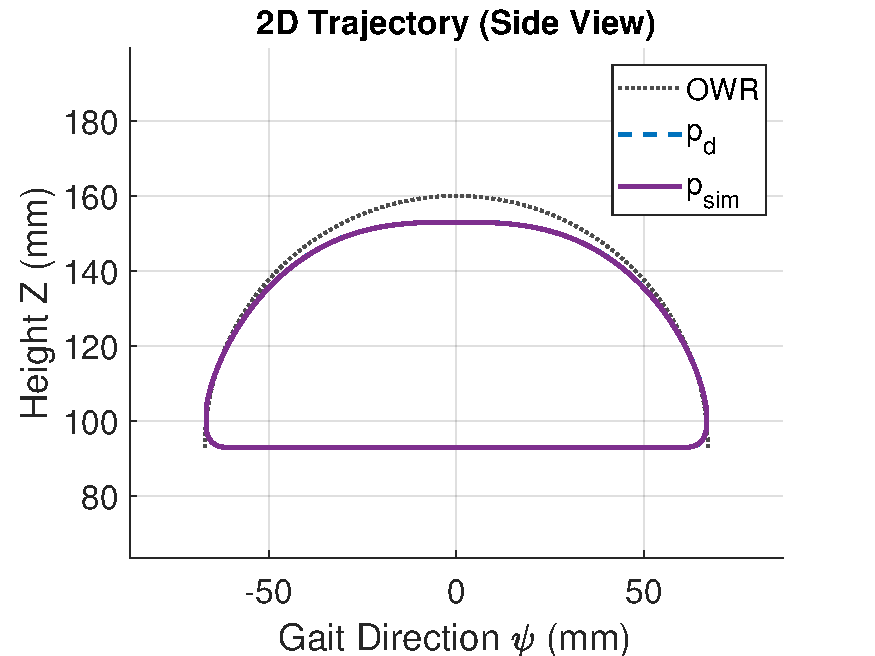
\includegraphics[width=0.65\textwidth]{images/gait_z_psi.pdf}
    \caption{Simulated Gait Ttrajectory in the $Z\psi$-plane (Side View).}
    \label{fig:gait_z_psi}
\end{figure}

The path clearly shows the linear stance phase (where Z is constant) and the smooth, $C^2$ continuous swing
phase, which lifts the foot to the required clearance height. Furthermore, the entire trajectory operates
correctly within the boundaries of the predefined Optimal Workspace Region (OWR).


\subsubsection{Cartesian Space Analysis}

A comprehensive overview of the system's performance in Cartesian space is depicted in Figure \ref{fig:cartesian_results}.

The three plots (X, Y, Z) demonstrate a perfect tracking of the commanded trajectory ($p_d$) as expected from the
ideal actuator assumption. The negligible errors ($e_{sim} \le 0.8\,mm$) are attributed to inertial effects
and a small tracking delay, both reasonable assumptions in real world systems.

\begin{figure}[htbp]
    \centering
    \begin{subfigure}[b]{0.8\textwidth}
        \centering
        
\includegraphics[width=\textwidth]{images/cartesian_trajectories.pdf}
        \caption{Trajectory Tracking}
    \end{subfigure}

    \begin{subfigure}[b]{0.8\textwidth}
        \centering
        
\includegraphics[width=\textwidth]{images/cartesian_errors.pdf}
        \caption{Tracking Errors}
    \end{subfigure}
    \caption{Cartesian-Space Simulation Results.}
    \label{fig:cartesian_results}
\end{figure}


\subsubsection{Joint Space Analysis}

Figure \ref{fig:joint_results} confirms that the Cartesian trajectory is correctly translated into smooth,
continuous joint commands, free of any "snaps" or sudden changes even at phase transition points.

Furthermore, all three trajectories operate comfortably within the designated joint limits, confirming the IK
solver is capable of finding a valid and safe solution.

\begin{figure}[htbp]
    \centering
    \begin{subfigure}[b]{0.8\textwidth}
        \centering
        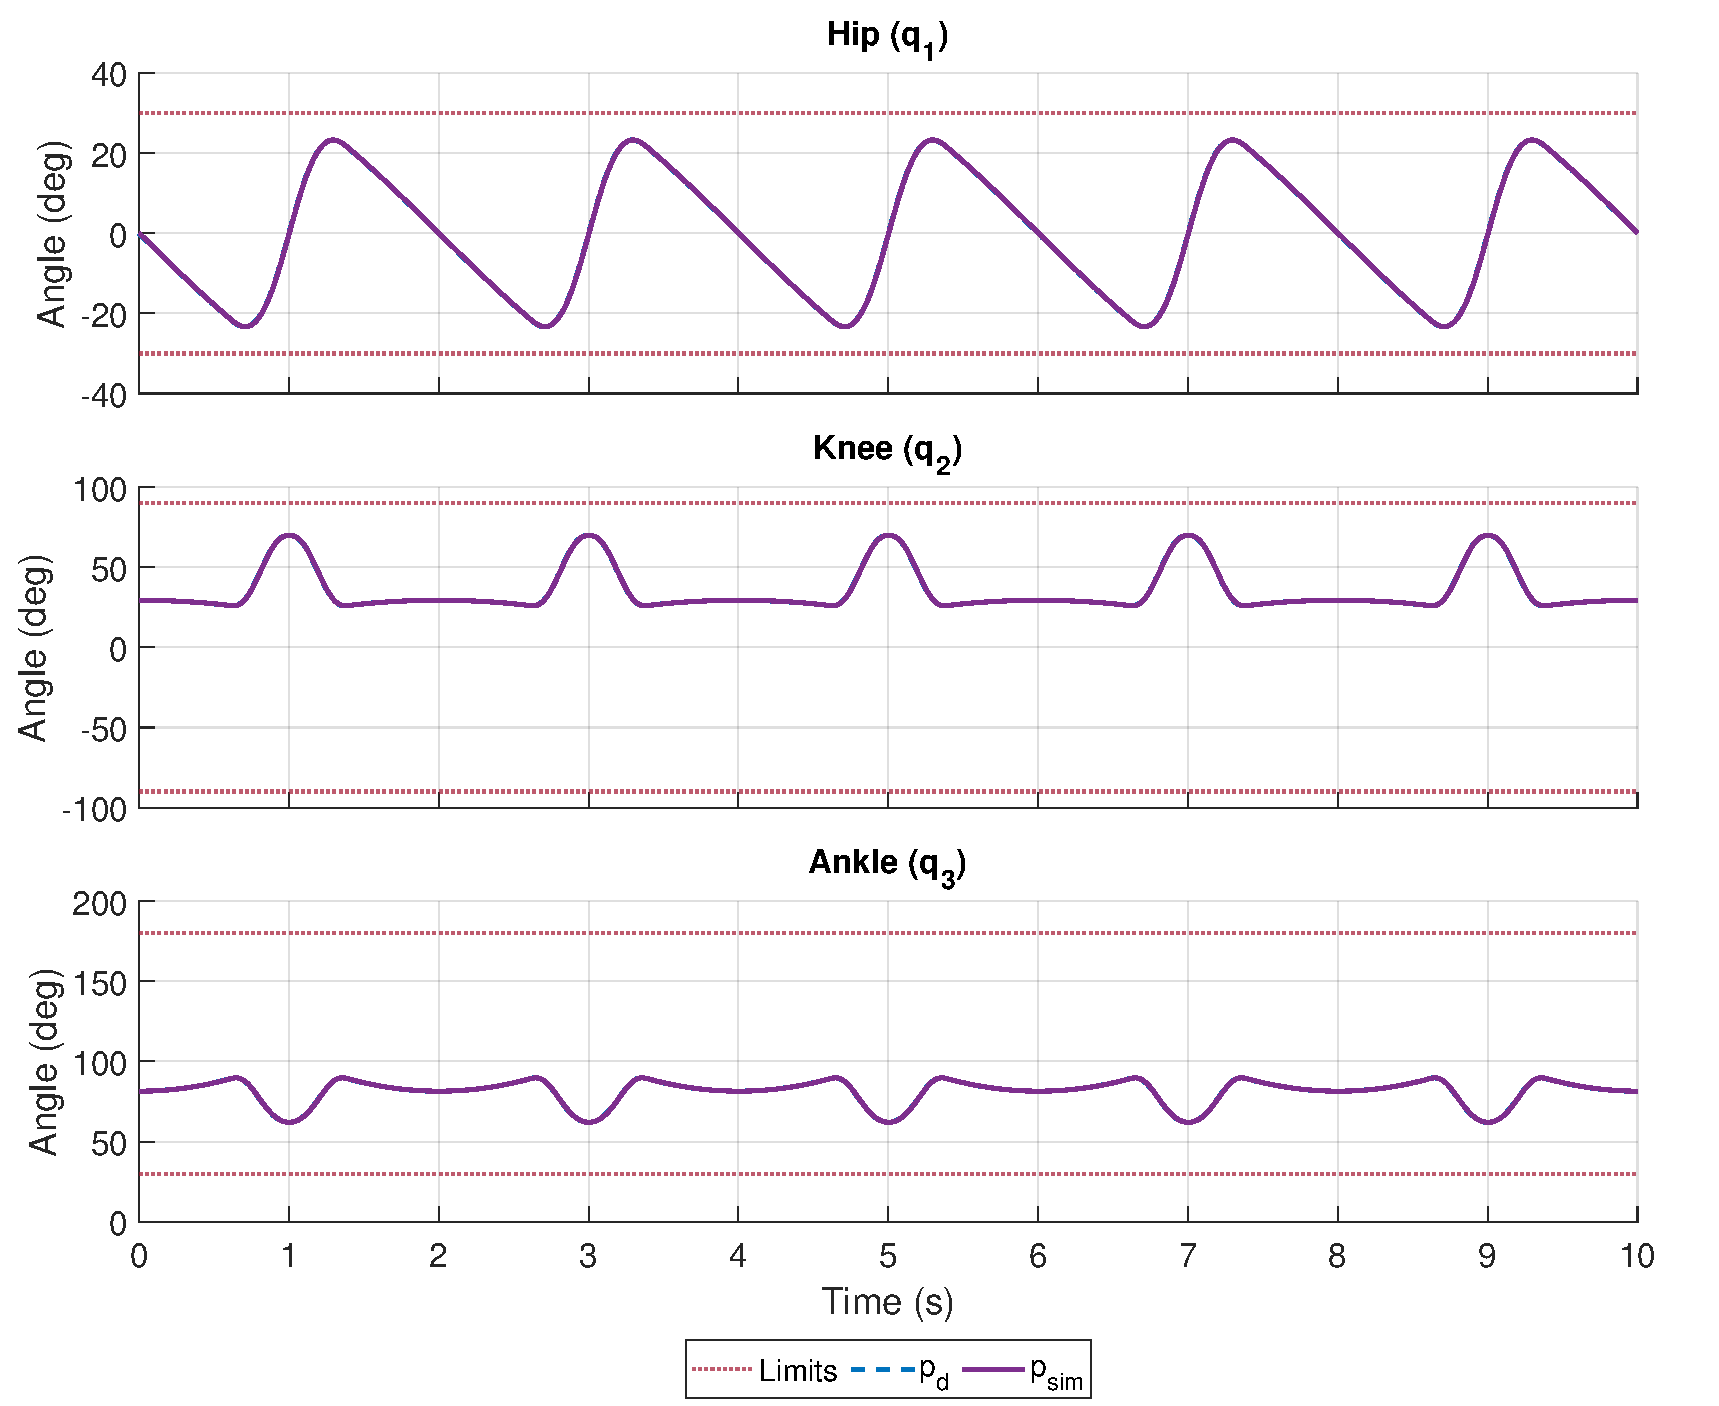
\includegraphics[width=\textwidth]{images/joint_trajectories.pdf}
        \caption{Trajectory Tracking}
    \end{subfigure}

    \begin{subfigure}[b]{0.8\textwidth}
        \centering
        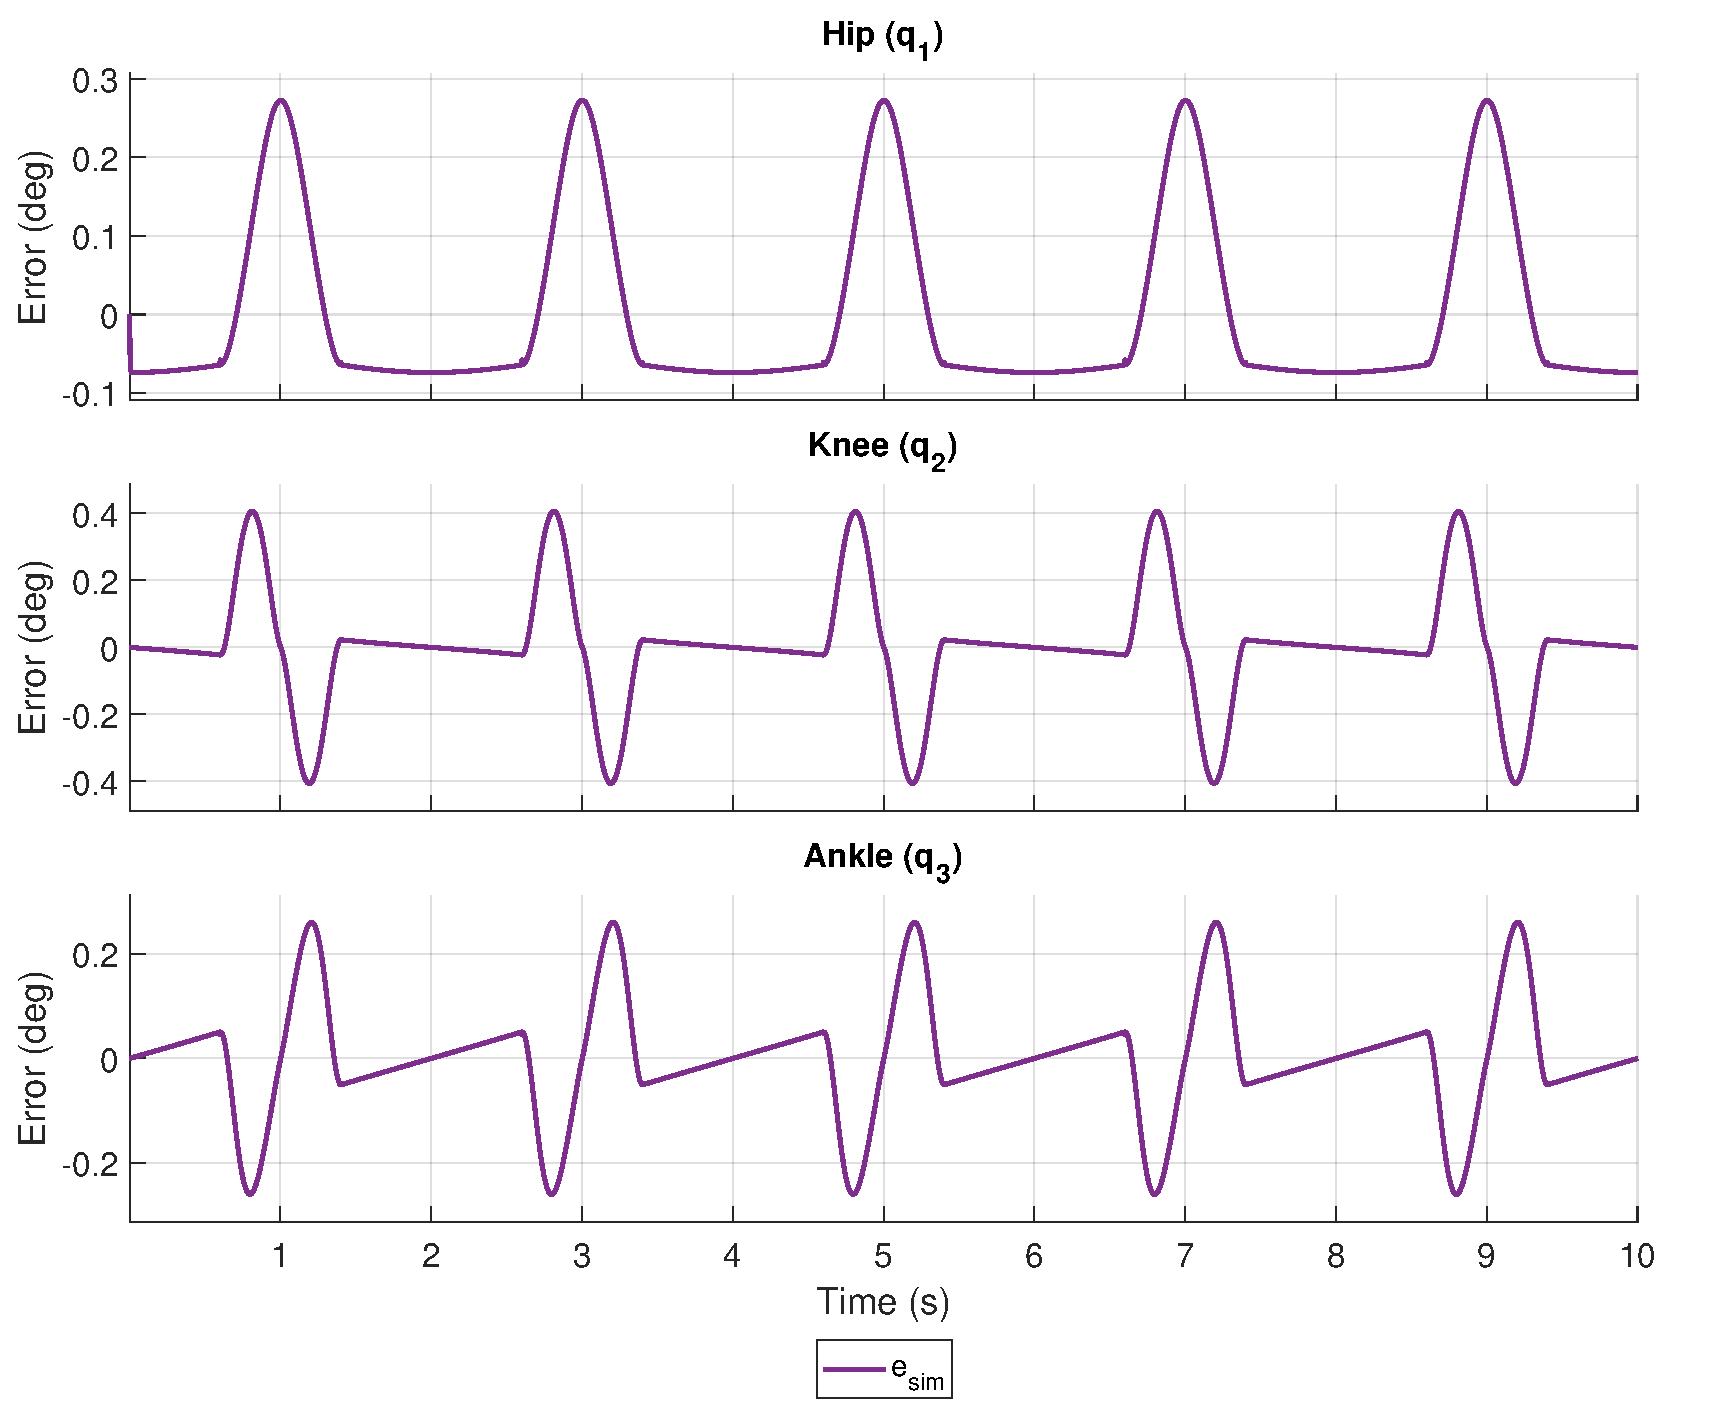
\includegraphics[width=\textwidth]{images/joint_errors.pdf}
        \caption{Tracking Errors}
    \end{subfigure}
    \caption{Joint-Space Simulation Results.}
    \label{fig:joint_results}
\end{figure}

\section{Proprioception and Path Adaptation}
\label{sec:proprioception}

The open-loop control strategy and kinematic chain validated in Section 2.2 demonstrated the system's theoretical
correctness under ideal conditions. However, this approach relies on the strict assumption of a perfectly flat
and predictable terrain ($z_{ground} = p_{z,0}$). In a real-world unstructured environment, ground elevation
varies unpredictably. Without feedback, a purely time-driven limb would either strike the ground prematurely
— causing high mechanical stress and potential instability — or fail to reach it entirely, compromising propulsion.

To relax this assumption and enable a "Blind Walking" \cite{brooks1989robot} capability, the system is
augmented with basic proprioceptive sensing and a reactive control layer. Admittedly, while this approach does
not fully solve the locomotion problem for extreme terrain (which would require a more structured control), it
represents the fundamental first step towards robust locomotion: the ability to detect and adapt to the ground
surface upon contact.


\subsection{Contact Sensing and Architectural Shift}

To detect the ground transition, the limb is equipped with a binary contact sensor located at the tip of the
foot. This sensor acts as a logical limit switch, providing a boolean signal $S_c$ to the controller:

$$
  S_c =
  \begin{cases}
    1 & \text{if touching ground}\\
    0 & \text{otherwise}
  \end{cases}
$$

The introduction of this sensor demands a fundamental shift in the control architecture. The path planning
problem transforms from a purely time-dependent function, $p_d(t)$, to a state-dependent system driven by
discrete events.

In the previous open-loop model, the gait phase was dictated by a global clock. In this adaptive model, the
controller must monitor $S_c$ and be capable of interrupting the Swing Phase exactly at the moment of
physical impact. Consequently, the trajectory generator cannot simply map a normalized time $t \in [0,1]$ to a
position; it must be restructured to handle asynchronous events and variable phase durations.


\subsection{Finite State Trajectory Generator}

To implement this reactive logic robustly, a custom Finite State Machine (FSM, Figure \ref{fig:fsm_logic}) was designed
\cite{cruse1990mechanisms}. This generator decouples the logical phase of the leg from the global clock,
allowing for local adaptations while maintaining synchronization through a phase-advance mechanism.

\begin{figure}[htbp]
    \centering
    \begin{tikzpicture}[
        ->,                       % Freccia su tutti i percorsi
        >=Stealth,                % Stile punta freccia moderno
        node distance=3.5cm and 4.5cm, % Distanza verticale e orizzontale
        every state/.style={      % Stile globale per i cerchi degli stati
            draw=black,
            thick,
            fill=gray!10,
            minimum size=3cm,     % Dimensione fissa per cerchi uniformi
            align=center          % Permette "a capo" dentro i cerchi
        },
        thick                     % Linee spesse
    ]

    % --- Definizione degli Stati ---

    % 1. Stance 1 (Alto-Sinistra) - Stato Iniziale
    \node[state, initial left, initial text={Start}] (S1) {Posterior\\Stance\\(Stance 1)};

    % 2. Lift (Alto-Destra) - A destra di S1
    \node[state] (Lift) [right=of S1] {Lift\\(Early Swing)};

    % 3. Touch (Basso-Destra) - Sotto a Lift
    \node[state] (Touch) [below=of Lift] {Touch\\(Late Swing)};

    % 4. Stance 2 (Basso-Sinistra) - A sinistra di Touch (e sotto S1)
    \node[state] (S2) [left=of Touch] {Anterior\\Stance\\(Stance 2)};

    % --- Transizioni (Frecce) ---

    % 1. Stance 1 -> Lift (Freccia verso destra)
    \path (S1) edge node[above, align=center] {
        $p_h \le -r$
    } (Lift);

    % 2. Lift -> Touch (Freccia verso il basso)
    \path (Lift) edge node[right, align=left] {
        $t > T_{lift}$
    } (Touch);

    % 3. Touch -> Stance 2 (Freccia verso sinistra)
    \path (Touch) edge node[below, align=center] {
        $S_c = 1$ \\
        \textit{-- or --} \\
        $t > T_{swing}$
    } (S2);

    % 4. Stance 2 -> Stance 1 (Freccia verso l'alto)
    \path (S2) edge node[left, align=right] {
        $p_h = 0$
    } (S1);

    \end{tikzpicture}
    \caption{Finite State Machine for Adaptive Trajectory Generation.}
    \label{fig:fsm_logic}
\end{figure}


\subsubsection{State 1: Posterior Stance (Stance 1)}

The initial state of the cycle. Geometrically, it corresponds to the leg moving from the central rest
position ($p_h = 0$) towards the posterior limit of the workspace ($p_h = -r$).

\newpage
The horizontal velocity is constant ($\dot{p}_h = -v$). The position is calculated via a discrete-time
integrator, which is reset upon entering the state. The vertical position $z$ is held constant at the
previously detected ground level.

Upon entering this state, the system calculates a synchronization parameter, $\delta(k)$, to compensate for any
timing drift accumulated in the previous cycle $k-1$. Recalling the duty factor $\beta$, the parameter is calculated as:
\begin{equation}
  \delta(k) = \left(1 - \frac{\beta}{2}\right) - t - \delta(k-1)
\end{equation}
where $t$ is the normalized global time counter. This ensures that the leg remains synchronized with the
robot's gait rhythm, correcting for local timing variations.

The system transitions to the Lift state when the horizontal position reaches the posterior stroke limit
($p_h \le -r$).


\subsubsection{State 2: Lift Phase (Early Swing)}

This state represents the deterministic part of the swing phase, where the leg lifts off the ground to clear
potential obstacles.

The duration of this phase, $T_{lift}$, is dynamically calculated to absorb the phase error $\delta(k)$:
\begin{equation}
  T_{lift} = T_{touch} + \delta(k) = \frac{1-\beta}{2} + \delta(k)
\end{equation}
This variable duration is the mechanism that re-synchronizes the leg with the robot's global gait cycle.

A quintic polynomial moves the foot vertically from its current height to the clearance height $H_{lift}$ over
the duration $T_{lift}$, while another quintic polynomial starts repositioning the foot horizontally over the
duration $T_{swing} = T_{lift} + T_{touch}$.

The state transitions only when the timer exceeds the allocated time ($t > T_{lift}$), meaning the foot has
reached the desired clearence height.


\subsubsection{State 3: Touch Phase (Late Swing)}

This state governs the descent of the leg. Crucially, this is where proprioceptive feedback is expected to trigger.

The timer variable is adjusted to parametrize the descent polynomial $t' = t_{norm} - T_{lift}$, guiding the
foot from $H_{lift}$ back towards the nominal ground ($z = 0$) over a fixed duration $T_{touch} = (1-\beta)/2$.
The global timer is maintained to preserve continuity with the swing phase dynamics.

The system exits this state under two distinct conditions:

\begin{enumerate}
  \item \textbf{Time-out:} The time expires ($t' > T_{touch}$ or equivalently $t > T_{swing}$), implying the leg
    completed the full trajectory without contact (e.g. a hole or flat ground).
  \item \textbf{Early Contact:} The sensor triggers ($S_c = 1$). This indicates the ground is higher
    than expected (e.g. an obstacle).
\end{enumerate}

In both cases, the FSM immediately transitions to the next state.


\subsubsection{State 4: Anterior Stance (Stance 2)}

Following the touchdown, the leg enters the anterior portion of the stance phase, moving from the anterior limit
($+r$ or the early contact point) back towards the central rest position ($p_h = 0$).

The horizontal velocity returns to $-v$. The vertical position $z$ is locked at the specific height recorded at
the moment of the Touch $\to$ Anterior Stance transition. This allows the robot to walk "on top" of obstacles rather
than trying to push through them.

The cycle completes when the leg crosses the zero-point of the workspace ($p_h = 0$), triggering the transition
back to Posterior Stance. At this crossing, the cycle index $k$ increments, and the loop repeats.


\subsection{Adaptive Simulation Results}

To validate the proprioceptive controller, the Simscape environment was modified to include an uneven terrain
profile.

Figure \ref{fig:adaptive_results} provides a direct comparison between the nominal, time-based trajectory
and the reactive, adaptive trajectory generated by the FSM in the presence of uneven terrain. For visual
clarity, these plots represent the trajectory primitives defined in the $Z\psi$-plane.


\subsubsection{Vertical Adaptation}

The bottom plot (Vertical Trajectory) clearly demonstrates the effectiveness of the proprioceptive loop. When
the limb encounters a positive obstacle (represented by the gray terrain profile), the adaptive trajectory
deviates from the nominal path exactly at the moment of impact. Unlike the nominal reference, which would
attempt to drive the foot through the terrain, the adaptive system triggers an immediate transition from the Touch
Phase to the Stance Phase. The vertical position is subsequently maintained at the obstacle's height for the
duration of the propulsion stroke, effectively allowing the robot to walk on top of the irregularity rather than
pushing against it.

\begin{figure}[htbp]
    \centering
    
\includegraphics[width=0.98\textwidth]{images/adaptive_comparison.pdf}
    \caption{Adaptive Gait Simulation with the New FSM Trajectory Generator.}
    \label{fig:adaptive_results}
\end{figure}


\subsubsection{Synchronization and Phase Correction}

Despite the timing disturbances introduced by early ground contacts, the top plot (Horizontal Trajectory) shows
that the system maintains robust synchronization. While the early impact inevitably causes a minor phase lead
(visible as a slight horizontal shift between the purple and green waves), the trajectory does not drift
indefinitely. Instead, when the obstacle is no longer present, the cycle realigns with the non-adaptive ideal
trajectory. This proves that the phase synchronization mechanism successfully compensates for these delays in
subsequent cycles, keeping the limb's rhythm bounded and consistent with the global gait cycle.


\subsubsection{Continuity and Stability Considerations}

There is key consideration to address regarding the kinematic continuity at the impact point: while the
generated trajectory primitives are designed to be $C^2$ continuous, the very nature of the "Blind Walk"
implies that the exact moment of touchdown is unpredictable. Consequently, when the ground is struck earlier
than planned, the vertical velocity changes abruptly from the descent speed to zero (relative to the terrain).
Therefore, at these specific transition points, strict $C^2$ continuity cannot be guaranteed.

Secondly, while effective as a proof of concept, this adaptive generator has specific limitations. For starters,
it currently compensates only for elevated obstacles (protrusions), neglecting potential depressions or holes
in the terrain. Also, unlike the nominal generator, this reactive strategy does not inherently guarantee that
the modified path remains within the Optimal Workspace Region (OWR); without explicit saturation limits, the
adaptation could potentially request kinematically unfeasible positions.

Another important consideration to keep in mind is the dynamic shortening of the foot's contact time introduces
significant stability challenges; therefore, a rigorous balance study is essential for the future implementation
of the full robot.

In summary, this strategy is designed specifically to handle minor terrain irregularities (roughness) rather
than large obstacles, representing a solid foundation for higher level obstacle avoidance planning and control
\cite{saranli2001rhex}.